\chapter{Implementación del modelo}
Este capítulo está dedicado a cubrir los detalles de la implementación del modelo en código, concretamente en lenguaje C++.

Dado que la principal finalidad de este trabajo es el modelado físico, no entraré en detalles en otras áreas del programa más que las que tienen que ver con lo descrito en los capítulos anteriores.

El programa completo contiene módulos para la graficación en \href{http://www.opengl.org/}{OpenGL}, para la interfaz de usuario por medio de \href{https://github.com/ocornut/imgui}{dear imgui}, para la lectura y escritura de imágenes usando \href{http://freeimage.sourceforge.io/}{freeimage} (para cargar texturas y para hacer capturas de pantalla) e implementa el modelo de iluminación de \href{http://en.wikipedia.org/wiki/Phong_reflection_model}{Phong} en shaders por medio de \href{http://www.khronos.org/opengl/wiki/OpenGL_Shading_Language}{GLSL}.

El lector interesado puede consultar el código fuente completo del programa que se incluye en un CD o puede descargarlo de \href{http://github.com/nemediano}{github}.
Aunque el código está escrito en inglés (por ser el estándar) traté de ser lo más extenso en los comentarios en todo el código.
Por lo que el lector que cuente con los conocimientos de programación y graficación por computadora adquiridos en la licenciatura podrá entender y usar todo el código fuente del programa sin ningún problema.

Se decidió implementar el programa usando el paradigma de programación orientada a objetos. 
En la primera sección se describen las clases más importantes: las necesarias para representar las estructuras del modelo y la clase que lleva a cabo la ejecución del programa.

La siguiente sección se revisa cómo se implementaron en código los métodos numéricos usados para integrar la ecuación de Newton.

En la tercera sección se explican las rutinas de la física del modelo, concretamente las rutinas que se encargan de aplicar las fuerzas que intervienen en el modelo.

En la última sección del capítulo, se explica cómo es que se implementaron la rutina tanto de detección como de respuesta a las colisiones.

\section{Diseño de clases}

Decidí usar de la biblioteca de algebra para graficos: \href{http://github.com/g-truc/glm}{glm} por dos razones.
Primero, por que cuenta con tipos de datos para representar vectores en 2 y 3 dimensiones e implementa las operaciones usuales entre ellos.
Y segundo, por que esta biblioteca tiene un alto nivel de integración con OpenGL al grado de ser casi un estandar.

La parte fundamental del modelo la constituyen las partículas; de cada una de éstas nos interesa saber básicamente cuatro cosas: su posición, su velocidad, la fuerza que se le está aplicando y la masa.
Adicionalmente, por un detalle particular a nuestra implementación, se necesita saber si una partícula esta fija.
Si una particúla esta fija, entonces se deben de ignorar las operaciones de integración.
Los métodos nos permiten editar y consultar estos cinco miembros. En este sentido la clase \mintinline{cpp}{Particle} es muy simple~\footnote{En el argot del lenguaje \href{http://www.java.com/en/}{Java} diriamos que la clase \mintinline{cpp}{Particle} es casi un \href{http://en.wikipedia.org/wiki/JavaBeans}{bean}}.

Para representar a los resortes-amortiguadores se creó la clase \mintinline{cpp}{SpringDamper} que tiene como miembros \emph{referencias} a las dos partículas que une éste resorte.
Hago énfasis en que usaremos referencias, pues las partículas van ser usadas para formar varios objetos y se requiere que no sea necesario actualizar en cada objeto por separado cada que una partícula sea modificada. Finalmente, se debe saber la longitud $L$ del resorte cuando está en su estado de reposo.

La clase \mintinline{cpp}{SpringDamper} tiene un define los métodos para:
\begin{itemize}
 \item Actualizar qué partículas forman éste resorte.
 \item Consultar y modificar $L$.
 \item Consultar las posiciones de las partículas que forman este resorte.
 \item Acumular la fuerza del resorte en sus dos partículas dados $k_s$ y $k_d$.
\end{itemize}

La última clase que define el cuerpo neumático es la clase \mintinline{cpp}{Face}, que representa una cara del cuerpo flexible.
Como es de esperar, dado que las caras son cuadriláteros, esta clase solo necesita como propiedades referencias a cuatro partículas.

Adicionalmente, la clase \mintinline{cpp}{Face} implementa los siguientes métodos:
\begin{itemize}
 \item Los accesores y mutadores a las partículas que la forman.
 \item Un método para actualizar las partículas que forman esta cara (equivalente al de \mintinline{cpp}{SpringDamper}).
 \item Un método para calcular el área de esta cara.
 \item Un método que sirve como auxiliar en el cálculo del volumen de todo el cuerpo flexible. La lógica de este método se explica en la Sección~\ref{sec:fuerzaGas}. Aunque ésta no es una propiedad de la cara, por razones de Ingeniería de Software (IS) era conveniente incluirlo en esta clase.
\end{itemize}

También se define una clase para representar el cuerpo flexible: \mintinline{cpp}{SoftBody}.
Esta clase es la más importante de la aplicación.
Y el resto de éste capítulo está dedicado a explicar como funcionan sus métodos.
En este momento, es relevante decir que esta clase contiene una colección de partículas, una colección de resortes y una colección de caras.
Las caras y resortes en realidad contienen referencias a las partículas, de esta manera la información de las partículas sólo está almacenada una vez.

Por orden, esta clase también define una estructura: \mintinline{cpp}{SoftBodyParameters} que contiene todos los parámetros físicos del cuerpo flexible. 
 
Finalmente, se necesita también una clase para representar el único cuerpo rígido en la escena.
La clase \mintinline{cpp}{Ball} tiene como miembros una partícula, un escalar que representa el radio de la esfera y un miembro para registrar qué método numérico se usa para integrar (De nuevo por IS, era conveniente que cada objeto en la escena llevará registro de que integrador está en uso).

La relación entre estas clases esta resumida en el diagrama de clases mostrado en la Figura~\ref{clases:fig}. De nuevo hago énfasis en que la implementación de hecho contiene mas miembros que los mostrados, pues solo aparecen en el diagrama los relevantes para este trabajo.

\begin{figure}
 \centering
 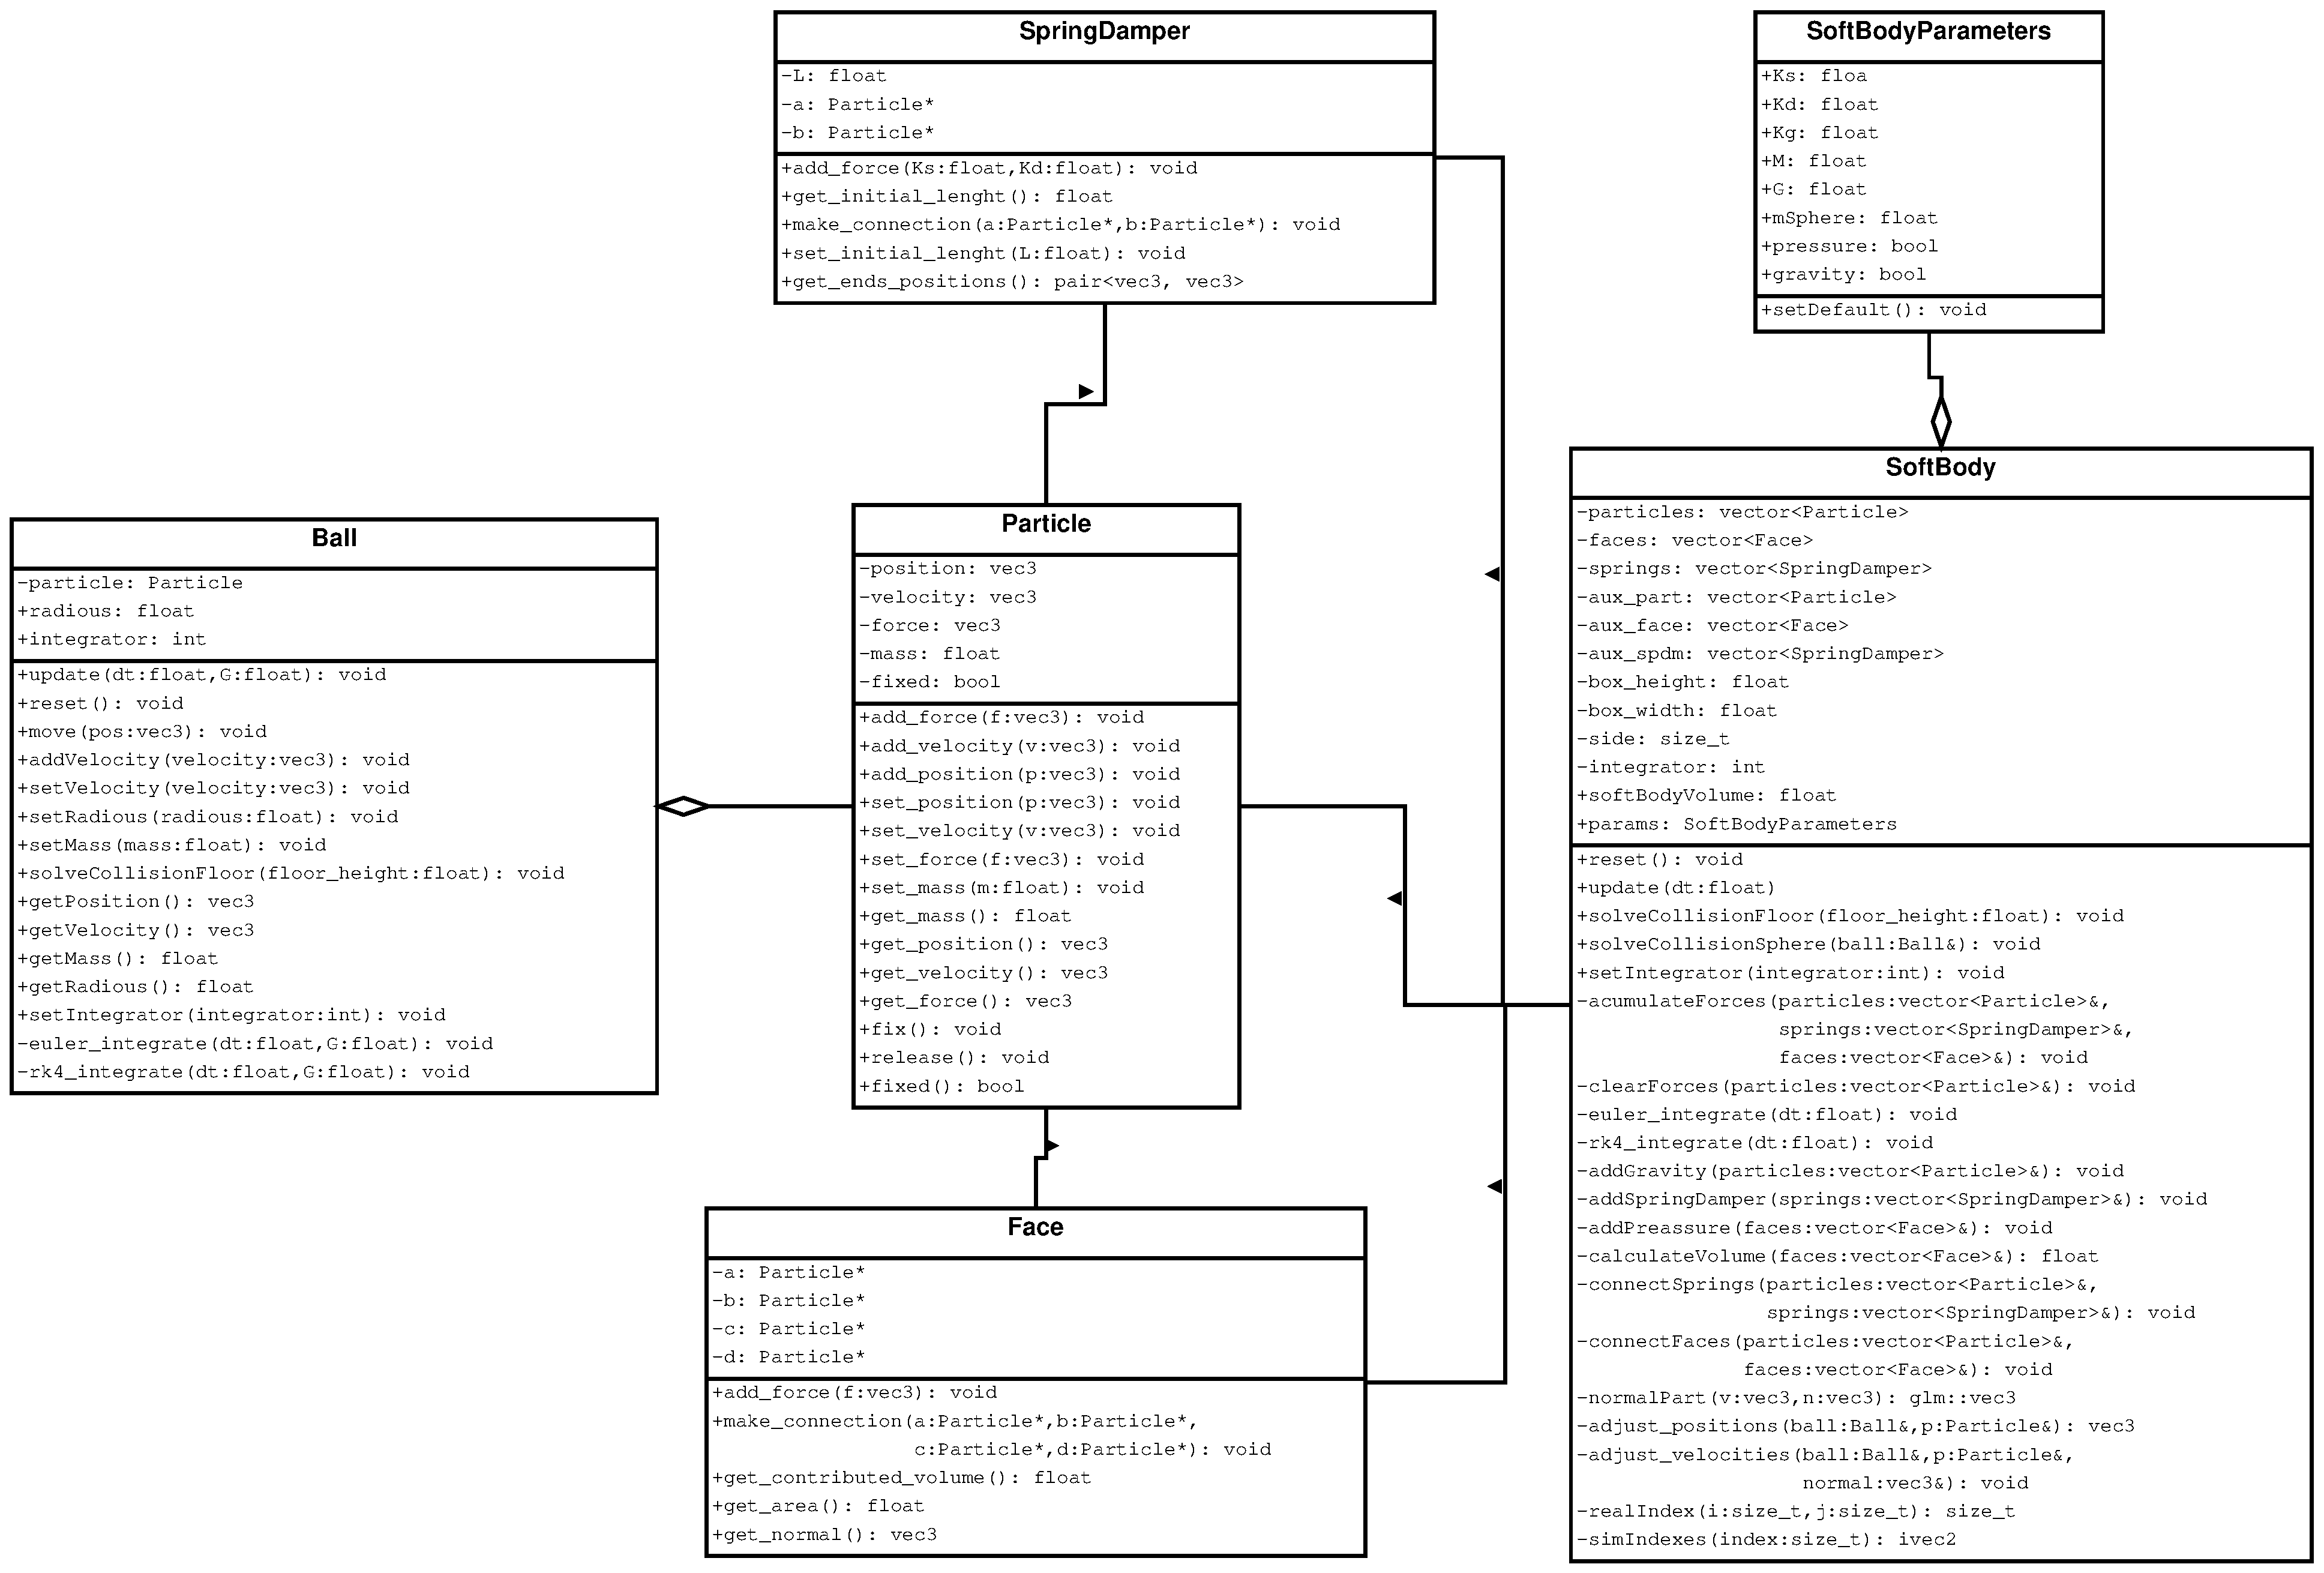
\includegraphics[width=\textwidth]{Img/03/diagramaClases}
 \caption[Diagrama de clases]{ 
 La clase \mintinline{cpp}{Particle} es la unidad de construcción. La clase \mintinline{cpp}{SoftBody} es la que controla la ejecución. 
 } \label{clases:fig}
\end{figure}

\section{Creación del cuerpo flexible}

Cómo se dijo en la sección anterior, hay tres colecciones que forman el cuerpo flexible: las particulas, los resortes y las caras. Estas colecciones estan almacenadas en vectores que forman parte de la clase \mintinline{cpp}{SoftBody}.

Hay algunas cosas que decir aquí: primero, que lo que se quiere modelar es una tela cuadrada que servirá como cuerpo flexible, por lo que el número de partículas es en realidad $n^{2}$ en donde $n$ es el número de puntos en cada lado de la tela (en el código es el miembro \mintinline{cpp}{size_t m_side} de \mintinline{cpp}{SoftBody}), y como no hay resortes en las orillas de la tela el número de resortes totales es $2 (n - 1) (n - 2)$ y el número de caras es: $(n-1)^{2}$.
Segunda, que, pese al arreglo cuadrado de la tela, los puntos son guardados en un arreglo unidimensional (lineal), esto por que simplifica y hace mucho más generales las rutinas de acumulación de fuerza.

Dado que la partículas están en un arreglo unidimensional se hace uso del método \mintinline{cpp}{simIndexes} que recibe el índice de la particula en el vector unidimensional y nos regresa los indices $(i, j)$ que la partícula tendría en un arreglo bidimensional. El metodo \mintinline{cpp}{realIndex} hace la operacion inversa.

La rutina que inicializa las partículas es la siguiente:

{\centering
\begin{minipage}{\linewidth}
  \begin{listing}[H]
  \inputminted[
  xleftmargin=1.5cm,  %without this option line number goes wrong
  %frame=lines,
  framesep=0.5cm,
  baselinestretch=1.2,
  fontsize=\footnotesize,
  linenos,
  firstline=306, %If you omit this two fields, the whole file is pulled
  lastline=328
  ]{cpp}{../../../GLSamples/SoftBody/physics/SoftBody.cpp}
  \caption{Este es un extracto del método \mintinline{cpp}{recreate_particles} de \mintinline{cpp}{SoftBody}}
  \label{lst:recreate_particles}
  \end{listing}
\end{minipage}
\par
}

El código mostrado en el Listado~\ref{lst:recreate_particles} inicializa la velocidad, la fuerza y la masa de la partículas (la posición es inicializada con una rutina muy simple que esta fuera de la clase \mintinline{cpp}{SoftBody}). También se encarga de fijar las partículas que estan en las orillas de la tela.

La rutina que inicializa los resortes es ejecutada después de las particulas. Se muestra un extracto en el Listado~\ref{lst:connectSprings}.

{\centering
\begin{minipage}{\linewidth}
  \begin{listing}[H]
  \inputminted[
  xleftmargin=1.5cm,  %without this option line number goes wrong
  %frame=lines,
  framesep=0.5cm,
  baselinestretch=1.2,
  fontsize=\footnotesize,
  linenos,
  firstline=345, %If you omit this two fields, the whole file is pulled
  lastline=368
  ]{cpp}{../../../GLSamples/SoftBody/physics/SoftBody.cpp}
  \caption{Este es un extracto del método \mintinline{cpp}{connectSprings} de \mintinline{cpp}{SoftBody}}
  \label{lst:connectSprings}
  \end{listing}
\end{minipage}
\par
}

Por las condiciones que definimos en nuestra tela. 
\begin{center}
 \item Las partículas que están en las arístas superiores e inferiores no tienen un resorte horizontal entre ellas.
 \item Las partículas que están en las arístas izquierda y derecha no tienen un resorte vertical entre ellas.
\end{center} 

El algoritmo, pregunta si esta particula puede ser unida (por un resorte) con la partícula a su derecha, de ser así las conecta. Después, pregunta si debe ser unida con la particula abajo de ella, de ser así tambien es conectada.

La logica para formar las caras se presenta en el Listado~\ref{lst:connectFaces}: 
{\centering
\begin{minipage}{\linewidth}
  \begin{listing}[H]
  \inputminted[
  xleftmargin=1.5cm,  %without this option line number goes wrong
  %frame=lines,
  framesep=0.5cm,
  baselinestretch=1.2,
  fontsize=\footnotesize,
  linenos,
  firstline=372, %If you omit this two fields, the whole file is pulled
  lastline=389
  ]{cpp}{../../../GLSamples/SoftBody/physics/SoftBody.cpp}
  \caption{Este es un extracto del método \mintinline{cpp}{connectFaces} de \mintinline{cpp}{SoftBody}}
  \label{lst:connectFaces}
  \end{listing}
\end{minipage}
\par
}

Esta rutina es muy parecida a la anterior: recorre todas las particulas, si la partícula actual, tiene un partícula a su izquierda y otra partícula abajo, entonces se pueden tomar cuatro partículas (pues debe existir otra una partícula en diagonal) para formar una cara.

\section{La física del modelo}
Toca el turno de ver las rutinas que tienen que ver con la acumulación de fuerzas en el modelo.
Como se ha dicho antes hay básicamente tres fuerzas que se deben acumular, la de la gravedad, la de los resortes amortiguadores y la debida a la presión del gas.

Estas rutinas se encuentran en los archivos: fisica.c y fisica.h
\subsection{La fuerza de gravedad}
La primera y más sencilla de las fuerzas que vamos a poner es la de gravedad.
Como se dijo desde~\ref{fuerzaGravedad}, sólo depende de dos cosas de la masa del objeto y de la constante de gravedad, y además sólo afecta en un componente vectorial el componente $y$, del vector fuerza.

La fuerza de gravedad se aplica a cada una de las partículas del cuerpo flexible, por lo que es conveniente acumularla por medio del un arreglo que contenga todos los puntos del cuerpo flexible.
Aquí está la función que pone la fuerza de gravedad:
\begin{verbatim}
void putGravity(Punto ptos[PARTICULAS])
{
   int i;
   for (i = 0; i < PARTICULAS; i++)
   {
      ptos[i].fy += M * G;
   }

}
\end{verbatim} 
La función \verb|putGravity|, recibe como parámetro un arreglo de puntos, y acumula sobre cada uno de los puntos la fuerza de gravedad.

La constante \verb|M| es global y tiene la masa de cada una de las partículas, y la constante \verb|G|, también global contiene la constante de gravedad.
En palabras simples acumula la fuerza sobre cada punto usando la ecuación~\ref{fuerzaGravedad}.

¿Por qué mandar como parámetro el arreglo de puntos, si es una variable global? Bueno eso se debe a que la gravedad no siempre será aplicada sobre el arreglo en el que guardamos puntos con los que se dibuja la escena, debido a que los métodos numéricos de integración (en particular el Runge Kutta) van a requerir copias del arreglo de puntos para hacer cálculos, por lo que no siempre se le mandará el \emph{mismo} arreglo de puntos.

\subsection{La fuerza de los resortes}
Aquí es donde empezaremos a notar el porqué de la construcción de los demás arreglos.
Primero vamos a ver qué se debe de hacer en esta función: se debe de ciclar por todos los resortes que se encuentran en el modelo; cada resorte se debe ocupar la ecuación~\ref{fuerzaResorte}, para acumular la fuerza en los dos puntos que son unidos por ese resorte.
\begin{verbatim}
void putSpringForce(Resorte res[RESORTES])
{
  int i;
  float rX, rY, rZ, vX, vY, vZ, Fd, Fs, Fx, Fy, Fz, largo;

  for (i = 0; i < RESORTES; i++)
  {
    // La distancia entre los dos puntos
    largo = distancia(*res[i].a, *res[i].b);

    if (largo != 0.0)
    {
      // la diferencia de las posisciones
      rX = res[i].a->x - res[i].b->x;
      rY = res[i].a->y - res[i].b->y;
      rZ = res[i].a->z - res[i].b->z;

      // la diferencia de las velocidades
      vX = res[i].a->vx - res[i].b->vx;
      vY = res[i].a->vy - res[i].b->vy;
      vZ = res[i].a->vz - res[i].b->vz;

      /* Calculo de las fuerzas (escalares)*/
      Fd = Kd * (rX * vX + rY * vY + rZ * vZ) / largo;
      Fs = Ks * (largo - L);

      /* Pongo las fuerzas escalares en un vector */
      Fx = -(Fd + Fs) * (rX / largo);
      Fy = -(Fd + Fs) * (rY / largo);
      Fz = -(Fd + Fs) * (rZ / largo);

      //Actualizo con la fuerza que acabo de calcular
      //El primer punto
      res[i].a->fx += Fx;
      res[i].a->fy += Fy;
      res[i].a->fz += Fz;

      //El segundo punto
      res[i].b->fx -= Fx;
      res[i].b->fy -= Fy;
      res[i].b->fz -= Fz;
    }
 }
}
\end{verbatim} 
Como se puede ver en el código, ahora ciclamos por todo el arreglo de resortes, y con ellos podemos acceder a los dos puntos \verb|a| y \verb|b| que conectan.
Lo primero es saber la distancia entre los dos puntos, si ésta fuera cero, no se hace ningún cálculo.
Cabe señalar que por las condiciones del modelo es muy difícil que dicho caso suceda.

Después se procede a calcular la fuerza del amortiguador y del resorte, para cada una de ellas se ocupan sus respectivas constantes \verb|Ks| y \verb|Kd|, que son variables globales.

Por último se le da la dirección a la fuerza del resorte y se actualiza en los puntos, recordando cambiar el signo en el segundo punto.
Hay también que hacer énfasis en que la fuerza nunca es actualizada directamente sino más bien es acumulada (sumada a la fuerza anterior).

\subsection{La fuerza del gas}
\label{sec:fuerzaGas}

La siguiente fuerza en ser acumulada es la fuerza debida a la presión del gas. Para esto se ocupa la ecuación~\ref{fuerzaGas}, y se debe de acumular una vez por cada cara.
Para poder calcular esta fuerza se necesitan hacer varias operaciones importantes: calcular el volumen total del cuerpo flexible y además calcular el área y el vector normal de cada una de las caras.

Para hacer el cálculo del volumen se hace uso de un arreglo de puntos auxiliares, se simula que el cuerpo está formado por varios pedazos rectangulares.
Para cada parte (hexaedro regular) se ocupa la fórmula~\ref{ecuacionVolumen} y finalmente la suma del volumen de todas nos proporciona el volumen total del cuerpo.

Para calcular el área de cada cara se ocupa la fórmula~\ref{formulaArea}.

Para calcular el vector normal se hace uso de la fórmula~\ref{formulaVecNormal}, en donde $n=4$, dado que cada cara está formada por cuatro puntos.

\begin{verbatim}
void putPressure (Punto pts[PARTICULAS], Cara msc[CUADROS])
{
  int i;
  float volumen = 0.0f, area, fuerza, largo, Fx, Fy, Fz;
  float vec1[3], vec2[3], vec3[3], vec4[3], vecPro[3];
  Punto aux[PARTICULAS];

  /* Puntos auxiliaes que me ayudaran a calcular el volumen */
  for (i = 0; i < PARTICULAS; i++)
  {
    aux[i].x = pts[i].x;
    aux[i].y = FONDO;
    aux[i].z = pts[i].z;
  }

  /** Calculo el volumen del cuerpo */
  for (i = 0; i < (LADO * (LADO - 1)); i++)
  {
    if ( (i % LADO) != (LADO - 1) )
    {
      volumen += volumenHexaedro(pts[i], pts[i+1], pts[i+LADO], 
      pts[i+1+LADO], aux[i], aux[i+1], aux[i+LADO], aux[i+1+LADO]);
    }
  }

  /** Loop sobre todas las caras para calcular su fuerza de presion */
  for (i = 0; i < CUADROS; i++)
  {
    /* El area de esta cara */
    area = areaCuadrilatero(*msc[i].a, *msc[i].b, *msc[i].c, *msc[i].d);

    fuerza = area * Kp / volumen;

    /* Calculo el vector normal a la cara */
    vectorNormal(*msc[i].a, *msc[i].c, *msc[i].b, vec1);
    vectorNormal(*msc[i].b, *msc[i].a, *msc[i].d, vec2);
    vectorNormal(*msc[i].c, *msc[i].d, *msc[i].a, vec3);
    vectorNormal(*msc[i].d, *msc[i].b, *msc[i].c, vec4);

    vecPro[0] = (vec1[0] + vec2[0] + vec3[0] + vec4[0]) / 4.0f;
    vecPro[1] = (vec1[1] + vec2[1] + vec3[1] + vec4[1]) / 4.0f;
    vecPro[2] = (vec1[2] + vec2[2] + vec3[2] + vec4[2]) / 4.0f;

    /* Hago unitario al vector normal */
    largo = sqrt(vecPro[0] * vecPro[0] + 
    vecPro[1] * vecPro[1] + vecPro[2] * vecPro[2]);

    msc[i].nx = vecPro[0] / largo;
    msc[i].ny = vecPro[1] / largo;
    msc[i].nz = vecPro[2] / largo;

    /* Calculo los vectores de fuerza */
    Fx = msc[i].nx * fuerza;
    Fy = msc[i].ny * fuerza;
    Fz = msc[i].nz * fuerza;

    /* Acomulo la fuerza de presion en cada particula de la cara */
    msc[i].a->fx += Fx;
    msc[i].a->fy += Fy;
    msc[i].a->fz += Fz;

    msc[i].b->fx += Fx;
    msc[i].b->fy += Fy;
    msc[i].b->fz += Fz;

    msc[i].c->fx += Fx;
    msc[i].c->fy += Fy;
    msc[i].c->fz += Fz;

    msc[i].d->fx += Fx;
    msc[i].d->fy += Fy;
    msc[i].d->fz += Fz;
  }
}
\end{verbatim}
Para calcular la fuerza de nuevo se hace uso de una variable global \verb|Kp|, que guarda la constante de la presión.
Y finalmente la fuerza se acumula en cada uno de los cuatro puntos que forman la cara.
También hay que notar que el vector normal a ésta se quedó guardado en \verb|nx|, \verb|ny| y \verb|nz|; después se puede hacer uso de él para hacer la iluminación de la escena.

La funciones \verb|volumenHexaedro| y \verb|areaCuadrilatero|, sólo hacen uso de las fórmulas~\ref{ecuacionVolumen} y~\ref{formulaArea}, respectivamente, y devuelven un valor real.

\section{Los métodos numéricos}
Otra de las rutinas mas complicadas son los métodos numéricos.
Para integrar la ecuación de Newton, se requiere saber la posición y la velocidad actual de cada una de las partículas del modelo y tener una manera de llamar a la función que se encarga de acumular las fuerzas.

\subsection{El método de Euler}
Básicamente se trata de tomar las ecuaciones~\ref{formulas:Euler} e implementarlas en el código, aprovechando la gran ventaja de que el método de Euler puede integrar un punto a la vez.
La función que se explica recibe de parámetro una referencia a un objeto de tipo \verb|Punto|.
\begin{verbatim}
void eulerIntegrator (Punto *p)
{
  float drx, dry, drz;

  /* Para las x */
  p->vx += p->fx / M * DT;
  drx = p->vx * DT;
  /* Para las y */
  p->vy += p->fy / M * DT;
  dry = p->vy * DT;
  /* Para las z */
  p->vz += p->fz / M * DT;
  drz = p->vz * DT;


  if (!p->fixed)
  {
    /* Ahora si los tengo que mover */
    p->x += drx;
    p->y += dry;
    p->z += drz;
  }
  else
  {
    p->vx = 0.0;
    p->vy = 0.0;
    p->vz = 0.0;

    p->fx = 0.0;
    p->fy = 0.0;
    p->fz = 0.0;
  }
}
\end{verbatim} 
Como puede apreciarse, esta función es muy sencilla, calcula con la fórmula~\ref{formulas:Euler} y guarda esos valores en variables.
Luego pregunta si el punto que le mandaron por referencia tiene el estado \verb|fixed|, de ser así, borra las fuerzas y las velocidades; en caso contrario, simplemente le aumenta el avance en este paso de tiempo. \verb|DT| es una constante real que guarda el tamaño del paso $h$.

\subsection{El método de Runge-Kutta}
Aquí se explica el que fue probablemente el método mas complicado de implementar, pues no tiene la ventaja de Euler de integrar cada partícula independientemente, así que necesita integrar todas juntas.
Además, debe tener espacio para guardar los ponderadores del paso de integración de cada partícula.

Para tener una idea clara de lo que que hace el siguiente código conviene volver a ver las ecuaciones~\ref{ponderadores:RK4} y~\ref{formulas:RK4}.
\begin{verbatim}
void rungeKuttaIntegrator (void)
{
  int i;

  float drx, dry, drz, dvx, dvy, dvz,
  k1[3][PARTICULAS], k2[3][PARTICULAS], k3[3][PARTICULAS], k4[3][PARTICULAS],
  l1[3][PARTICULAS], l2[3][PARTICULAS], l3[3][PARTICULAS], l4[3][PARTICULAS];
  /*La segunda dimension es el numero de puntos en la tela */

  Punto auxPun[PARTICULAS];
  Resorte auxRes[RESORTES];
  Cara auxCar[CUADROS];

  /*Inicializa los resortes auxiliares, para que apunten a 
    los puntos auxiliares y podamos llamar a la funcion 
    acumulate forces sobre ellos */
  ponResortes(auxPun, auxRes);
  ponCaras(auxPun, auxCar);

  /* Calculo ponderadores de primer orden K1 y L1 */
  for (i = 0; i < PARTICULAS; i++)
  {
     k1[0][i] = tela[i].fx / M;
     l1[0][i] = tela[i].vx;

     k1[1][i] = tela[i].fy / M;
     l1[1][i] = tela[i].vy;

     k1[2][i] = tela[i].fz / M;
     l1[2][i] = tela[i].vz;
  }
//===================================================================
  /* Copio en los auxPun para poder estimar una fuerza media */
  for (i = 0; i < PARTICULAS; i++)
  {
     auxPun[i].x  = tela[i].x  + (DT / 2.0f) * l1[0][i];
     auxPun[i].y  = tela[i].y  + (DT / 2.0f) * l1[1][i];
     auxPun[i].z  = tela[i].z  + (DT / 2.0f) * l1[2][i];

     auxPun[i].vx = tela[i].vx + (DT / 2.0f) * k1[0][i];
     auxPun[i].vy = tela[i].vy + (DT / 2.0f) * k1[1][i];
     auxPun[i].vz = tela[i].vz + (DT / 2.0f) * k1[2][i];
  }

  acomulateForces(auxPun, auxRes, auxCar);

  /* Calculo ponderadores de segundo orden K2 y L2 */
  for (i = 0; i < PARTICULAS; i++)
  {
     k2[0][i] = auxPun[i].fx / M;
     l2[0][i] = auxPun[i].vx + (DT / 2.0f) * k1[0][i];

     k2[1][i] = auxPun[i].fy / M;
     l2[1][i] = auxPun[i].vy + (DT / 2.0f) * k1[1][i];

     k2[2][i] = auxPun[i].fz / M;
     l2[2][i] = auxPun[i].vz + (DT / 2.0f) * k1[2][i];
  }

//=============================================================
  /* Copio en los auxPun para poder estimar una fuerza media */
  for (i = 0; i < PARTICULAS; i++)
  {
     auxPun[i].x  = tela[i].x  + (DT / 2.0f) * l2[0][i];
     auxPun[i].y  = tela[i].y  + (DT / 2.0f) * l2[1][i];
     auxPun[i].z  = tela[i].z  + (DT / 2.0f) * l2[2][i];

     auxPun[i].vx = tela[i].vx + (DT / 2.0f) * k2[0][i];
     auxPun[i].vy = tela[i].vy + (DT / 2.0f) * k2[1][i];
     auxPun[i].vz = tela[i].vz + (DT / 2.0f) * k2[2][i];
  }

  acomulateForces(auxPun, auxRes, auxCar);

  /* Calculo ponderadores de tercer orden K3 y L3 */
  for (i = 0; i < PARTICULAS; i++)
  {
     k3[0][i] = auxPun[i].fx / M;
     l3[0][i] = auxPun[i].vx + (DT / 2.0f) * k2[0][i];

     k3[1][i] = auxPun[i].fy / M;
     l3[1][i] = auxPun[i].vy + (DT / 2.0f) * k2[1][i];

     k3[2][i] = auxPun[i].fz / M;
     l3[2][i] = auxPun[i].vz + (DT / 2.0f) * k2[2][i];
  }

//=============================================================
   /* Copio en los auxPun para poder estimar una fuerza media */
  for (i = 0; i < PARTICULAS; i++)
  {
     auxPun[i].x  = tela[i].x  + DT * l3[0][i];
     auxPun[i].y  = tela[i].y  + DT * l3[1][i];
     auxPun[i].z  = tela[i].z  + DT * l3[2][i];

     auxPun[i].vx = tela[i].vx + DT * k3[0][i];
     auxPun[i].vy = tela[i].vy + DT * k3[1][i];
     auxPun[i].vz = tela[i].vz + DT * k3[2][i];
  }

  acomulateForces(auxPun, auxRes, auxCar);

  /* Calculo ponderadores de cuarto orden K4 y L4 */
  for (i = 0; i < PARTICULAS; i++)
  {
     k4[0][i] = auxPun[i].fx / M;
     l4[0][i] = auxPun[i].vx + DT * k3[0][i];

     k4[1][i] = auxPun[i].fy / M;
     l4[1][i] = auxPun[i].vy + DT * k3[1][i];

     k4[2][i] = auxPun[i].fz / M;
     l4[2][i] = auxPun[i].vz + DT * k3[2][i];
  }
//=======================================================================

  for(i = 0; i < PARTICULAS; i++)
  {
     if (!tela[i].fixed)//if que checa que el punto no este fijo
     {
        /* Calculo los incrementos */
        dvx = (DT/6.0f)*(k1[0][i]+2.0f*(k2[0][i]+k3[0][i])+k4[0][i]);
        drx = (DT/6.0f)*(l1[0][i]+2.0f*(l2[0][i]+l3[0][i])+l4[0][i]);

        dvy = (DT/6.0f)*(k1[1][i]+2.0f*(k2[1][i]+k3[1][i])+k4[1][i]);
        dry = (DT/6.0f)*(l1[1][i]+2.0f*(l2[1][i]+l3[1][i])+l4[1][i]);

        dvz = (DT/6.0f)*(k1[2][i]+2.0f*(k2[2][i]+k3[2][i])+k4[2][i]);
        drz = (DT/6.0f)*(l1[2][i]+2.0f*(l2[2][i]+l3[2][i])+l4[2][i]);

        /* Ahora si los tengo que mover */
        tela[i].x  += drx;
        tela[i].vx += dvx;

        tela[i].y  += dry;
        tela[i].vy += dvy;

        tela[i].z  += drz;
        tela[i].vz += dvz;
     }
     else //esta fijo velocidades y fuerzas a cero
     {
        tela[i].vx = 0.0f;
        tela[i].vy = 0.0f;
        tela[i].vz = 0.0f;

        tela[i].fx = 0.0f;
        tela[i].fy = 0.0f;
        tela[i].fz = 0.0f;
     }
   }
}
\end{verbatim}
El truco consiste en ocupar un conjunto de puntos, resortes y caras auxiliares, para con ellos calcular los ponderadores del método de RK4, después la rutina es muy parecida a la de Euler.

\section{El manejo de las colisiones}
Como ya se ha dicho antes, el problema de las colisiones se resuelve en dos partes, primero la detección y luego la respuesta.
La forma de responder consiste básicamente en mover los objetos que se colisionan a un lugar donde ya no choquen y ajustar las velocidades como respuesta.

\subsection{La rutina de las colisiones}
La detección es llevada a cabo en dos funciones.
Recordemos que nuestra tarea de detección se simplifica muchísimo por el hecho de que uno de los objetos, el objeto incidente es una esfera.
Para saber si dicha esfera está en colisión con nuestro cuerpo flexible, lo que hacemos es probar si cualquiera de las partículas está dentro de la esfera; de ser así, empezamos a resolver la colisión entre la esfera y la partícula en cuestión. Después seguimos revisando el resto de las partículas.

El algoritmo tiene la siguiente forma:
\begin{verbatim}
void colisiones (void)
{
  int i;
  Vector n;

  for (i = 0; i < PARTICULAS; i++)
  {
    if (dentro(tela[i]))
    {
      n = detectaColision(&tela[i]);
      respondeColision(&tela[i], n);
    }
  }
}
\end{verbatim}
Recordemos que \verb|tela|, es un arreglo global que contiene todos los puntos, se hace un ciclo por todo este arreglo preguntando con la función \verb|dentro| si está adentro de la esfera; de ser así, se manda llamar la funcion que detecta la colisión, es decir calcula el vector normal y lo devuelve.
Luego ese vector normal \verb|n| y el punto son mandados a la función que resuelve la colisión. Y así sucesivamente con todas las partículas que forman parte del cuerpo flexible.

La función \verb|dentro|, sabe si hay una colisión, pues la esfera está guardada en una variable global y el punto se le pasa como parámetro, así que sólo regresa verdadero cuando la distancia del punto al centro de la esfera es menos que el radio de ésta y falso en cualquier otro caso.

\subsection{La detección de la colisión}
Esta función se encarga de calcular el vector normal al lugar de la colisión y de mover el punto fuera de la esfera.
Mover el punto fuera de la esfera es en realidad parte de la respuesta a la colisión, pero decidí implementarlo en esta función, para que en la siguiente parte sólo se tenga que ajustar las velocidades.
\begin{verbatim}
Vector detectaColision(Punto *p)
{
  float vecV[3], distancia;
  Vector resultado, V;
  /* Obtenemos vector V que va del centro de la esfera al punto */
  V.x = p->x - pelota.x;
  V.y = p->y - pelota.y;
  V.z = p->z - pelota.z;
  /* Normalizamos V y lo guardamos en n, 
     N me sirve para hacer varios caluclos */
  distancia = sqrt((V.x * V.x) + (V.y * V.y) + (V.z * V.z));
  resultado.x = V.x / distancia;
  resultado.y = V.y / distancia;
  resultado.z = V.z / distancia;
  /* Movemos al punto fuera de la esfera, esto en realidad es parte 
   * de la respuesta, pero lo pongo aqui, para que en la respuesta 
   * solo ajuste las velocidades */
  if (!p->fixed)
  {
    p->x = pelota.x + (pelota.radio * resultado.x);
    p->y = pelota.y + (pelota.radio * resultado.y);
    p->z = pelota.z + (pelota.radio * resultado.z);	
  }
  else
  {
    pelota.x = p->x - (pelota.radio * resultado.x);
    pelota.y = p->y - (pelota.radio * resultado.y);
    pelota.z = p->z - (pelota.radio * resultado.z);
  }
  return resultado;
}
\end{verbatim} 
La función primero calcula el vector $\textbf{V}$ que va del centro de la esfera al punto, después lo normaliza.
Luego pregunta si el punto no está fijo, en cuyo caso, mueve el punto justo afuera de la esfera, cambiándolo de posición al punto $\textbf{p} + (r\textbf{V})$, donde $\textbf{p}$ es la posición de la esfera, $r$ su radio y $\textbf{V}$ ya es unitario. Si el punto sí estuviera fijo, lo que hace es mover a la esfera fuera del punto cambiándola de posición al punto $\textbf{s} - (r\textbf{V})$, donde $\textbf{s}$ ahora representa la posición de la partícula..

\subsection{La respuesta de la colisión}
La mayor parte del trabajo se hizo en la función anterior, ahora que sabemos el vector normal $\textbf{n}$ a la colisión, sólo nos resta seguir los pasos explicados en la página \pageref{alg:elasmov}.
\begin{verbatim}
void respondeColision (Punto *p, Vector normal)
{
  float r;
  Vector U, Un, Ut, Sn, Wn;

  r = Mp / M;

  U.x = pelota.Vx - p->vx;
  U.y = pelota.Vy - p->vy;
  U.z = pelota.Vz - p->vz;

  Un = parteNormal(U, normal);

  Ut.x = U.x - Un.x;
  Ut.y = U.y - Un.y;
  Ut.z = U.z - Un.z;

  Sn.x = Un.x * ( (r - 1.0f) / (r + 1.0f) );
  Sn.y = Un.y * ( (r - 1.0f) / (r + 1.0f) );
  Sn.z = Un.z * ( (r - 1.0f) / (r + 1.0f) );

  Wn.x = Un.x * ( (2.0f * r) / (r + 1.0f) );
  Wn.y = Un.y * ( (2.0f * r) / (r + 1.0f) );
  Wn.z = Un.z * ( (2.0f * r) / (r + 1.0f) );

  pelota.Vx = Ut.x + Sn.x + p->vx;
  pelota.Vy = Ut.y + Sn.y + p->vy;
  pelota.Vz = Ut.z + Sn.z + p->vz;

  p->vx = Wn.x + p->vx;
  p->vy = Wn.y + p->vy;
  p->vz = Wn.z + p->vz;
}
\end{verbatim}
En donde las constantes \verb|Mp| y \verb|M| tiene las masas de la esfera y de la partícula, respectivamente.
